\section{Evaluation}\label{sec_evaluation}
In this section, we evaluate our proposed hybrid \pso{} algorithms for the allocation of software applications to heterogeneous computing units, which conform to the system model presented in Section \ref{sec_system}. The algorithms are evaluated against different specifications of automotive software applications and execution platforms with regard to effectiveness, stability and scalability. The software-application specifications consist of the number of software components $c$, runnables $r$, tasks $t$ and cause-effect chains $g$.  The specifications are synthesized from the automotive benchmark proposed by Kramel et al.~\cite{Kramer2015RealFree}. The benchmark indicates a strong correlation between runnables and cause-effect chains in terms of timing and activation patterns. It shows the timing specifications of runnables and their shares in an engine management system. Moreover, it shows the activation patterns of cause-effect chains, the runnables per activation and their shares in the system. The engine management system is one of the most complex automotive systems in the vehicular electrical/electronic execution platform. 

\paragraph{Software Applications Benchmark} Based on our experience in the automotive industry, the benchmark results  are extrapolated to characterize different classes of automotive software application specifications, that is by varying the parameters related to the software components, runnables, and cause-effect chains. The different classes of specifications range from Spec-I to Spec-V as shown in Table~\ref{tbl_app_ranges}. The specification classes are useful to evaluate and discuss the effectiveness and scalability of the different optimization algorithms. The first specification class Spec-I encompasses small software applications with number of components less than 10, runnables less than 50, tasks 30, cause-effect chains less than 30. The Spec-I and Spec-II classes represent medium and large software applications, and the last specification class is introduced to stretch the performance analysis. 
\begin{table}
\centering\small
\begin{tabular}{@{}lllll@{}}
\toprule
Parameter  		& Spec.-I  & Spec.-II & Spec.-III & Spec.-IV\\
\midrule
Components $c$		& $\leq 10$	& $\leq 15$ 	&$\leq 20$ & $\leq 80$\\ 
Runnables $r$		& $\leq 50$	& $\leq 100$ 	& $\leq 500$&$\leq 1000$\\
Tasks $t$ 			& $\leq 30$ & $\leq 60$ 	& $\leq 80$&$\leq 100$\\
Cause-effect chains $g$ & $\leq$ 30 & $\leq$ 40 & $\leq 60$&$\leq100$\\ \midrule
Activation-pattern	& \multicolumn{4}{c}{$\{2,3,4\}$}\\ \midrule
share of activation-patterns	& \multicolumn{4}{c}{$\{0.7, 0.2, 0.1\}$}\\
\bottomrule
\end{tabular}
\caption{Specification of the Applications for Evaluation.}
\label{tbl_app_ranges}
\end{table}

\paragraph{Execution Platform Specifications}
Likewise, the specifications for an execution platform consist of the processor speed, power specifications and failure rates of computing units. The values of these parameters are shown in Table~\ref{tbl_execpla}.
\begin{table}
	\small
	\parbox{.4\linewidth}{
		\centering
		\begin{tabular}{@{}ll@{}}
			&\\&\\
			\toprule
			Parameter  			& Range\\ 
			\midrule
			\ttEE					 	& 100$n_\Gamma$\\
			\ttRL 						& 0.99999999\\
			\ttCL 						& \{A,B,C,D\}\\
			\bottomrule
		\end{tabular}
		\caption{Ranges of values for applications requirements.}
		\label{tbl_app_reqs_ranges}
	}
~
	\parbox{.6\linewidth}{
		\centering\raggedbottom
		\begin{tabular}{@{}ll@{}}
			\toprule
			Parameter  		& Range\\ 
			\midrule
			Nodes $n_N$							& $[4,10]$\\
			$P_{idle}$ (Watt)	& $[10,200]$\\
			$P_{busy}$ (Watt)	& $[20,500]$\\
			$\lambda_n,\lambda_B$ ($h^{-1}$) 	& $[10^{-8},10^{-6}]$\\
			$Hz$ & processor speed*\\
			\bottomrule
		\end{tabular}
		\caption{Ranges of values for execution platforms. \\Note: *~is reflected in the worst-case execution time.}
		\label{tbl_execpla}
	}
\end{table}

\paragraph{Applications Requirements Specifications} Table~\ref{tbl_app_reqs_ranges}  shows the range of values used in our experiments to specify the requirements of software applications, that include the end-to-end timing requirements (\ttEE) of chains, the reliability requirement (\ttRL) and the criticality level (\ttCL). The end-to-end requirements are assumed as a function of length of the chain $n_\Gamma$, i.e., the longer the chain the higher the number. The reliability range of a typical safety-critical automotive application is usually given in higher degree of 9, for operation of over a long period of time, which implies almost no failure during the specified duration.

\paragraph{Evaluation Setup} The evaluation is conducted on a MacBook Pro laptop computer, with hardware specifications as follows: Intel Core i7 processor type, 2.6.GHz processor speed, 6 Cores , 9 MB L3 cache, and 16 GB memory.

\subsection{Results}
We conducted two experiments: i) the first experiment is designed to compare the performance such as the convergence time, computation time, optimality (or quality of solutions) and stability of the meta-heuristic algorithms used in this paper, ii) the second experiment is designed to evaluate the overhead of increasing replication on the optimization especially due to the computation of end-to-end delays, and also to evaluate the effect of the approximation algorithm proposed in Subsection~\ref{subsec_approximation_alg} to reduce the overhead.
\begin{table}
	\centering\small
	\begin{tabular}{@{}lp{0.8\linewidth}@{}}
		\toprule
		Algorithm & Parameters Settings\\ 
		\midrule
		\pso	& Particle Swarm Optimization: learning factors $c_1=c_2=1.49445\in [0,4]$,  number of particles 40, iterations 5000	\\
		\de	& Differential Evolution: crossover $CR=0.5\in[0,1]$, scale factor $F=0.7\in[0,2]$  \\
		PF& Penalty Function:  $\beta_1=\mathcal{P}^{max}$,  $\beta_2=\mathcal{P}^{max}, \beta_3=10^8\mathcal{P}^{max}$, where  $\mathcal{P}^{max}=\sum_{i\in \mathcal{N}}{P_{busy_i}}$\\
		\bottomrule
	\end{tabular}
	\caption{Parameters settings of the metaheuristic optimization.}
	\label{tbl_para}
\end{table}

\paragraph{Experiment 1} Based on the ranges specifications presented in Table~\ref{tbl_app_reqs_ranges}, Table~\ref{tbl_app_ranges} and Table~\ref{tbl_execpla}, we synthesized six optimization problems as shown in Table~\ref{tbl_opt_problems}. The problems emulate the software allocation of safety-critical distributed automotive applications on heterogeneous computing units with respect to processor speed, failure rate and power consumption. The problems are identified by handlers of type $\langle c_ig_jn_i\rangle$ for readability, where the $c,g,n$ variables denote number of components, cause-effect chains and computing units, respectively. The \pb{6}{10}{4} and \pb{8}{20}{6} problems correspond to Spec-I, thus represent the allocation of small size software applications. The \pb{10}{20}{8} problem is based on Spec-II, thus denote the allocation of medium size software applications, and the \pb{20}{30}{10}, \pb{50}{40}{20} and \pb{80}{60}{20} are based on Spec-III, thus denote the allocation of large size software applications. The optimization problems are executed each 30$\times$ using our \ilp{} method proposed in \cite{Mahmud5222} and the meta-heuristic algorithms presented in Section~\ref{sec_solution}. The optimization parameters such as the penalty function coefficients and the meta-heuristic parameters control the optimization, and their settings are shown in Table~\ref{tbl_para}. The optimization parameter values are obtained from literature as well as from our experimentation. Subsequently, we recorded the computation time, fitness values and power consumption delivered by each algorithm.
\begin{table}
	\centering
	\begin{tabular}{@{}lllll@{}}
	\toprule
	Identifier &  Components $c$ &  Runnables $r$ &  Chains $g$&  Nodes $n$\\ 
	\midrule
	\pb{6}{10}{4} 		& 6 	& 60 & 10 & 4\\
	\pb{8}{20}{6}  		& 8     &80& 20 & 6 \\
	\pb{10}{20}{8}  	& 10   &100& 20 & 8 \\
	\pb{20}{30}{10}   & 20 	 & 200&30& 10 \\ 
	\pb{50}{40}{20}  & 50 	 &500& 60 & 20 \\
	\pb{80}{60}{20}  & 80	&800& 60 & 20 \\
	\bottomrule
\end{tabular}
\caption{Specifications of Optimization Problems.}
\label{tbl_opt_problems}
\end{table}
\paragraph{Experiment 2} Usually the replication exerts heavy computation over the calculations of the cause-effect delay due its combinatorial nature. The approximation technique, which is presented in Subsection~\ref{subsec_approximation_alg} optimizes the calculations of the cause-effect chain delay in the presence of replication. We executed the optimization problems \pb{50}{40}{20} and \pb{80}{60}{20} with 2 and 3 degrees of replication, and also with and without the approximation technique applied according to the specification in Table~\ref{tbl_samples}. The degree of replication indicates the multiplicity of each component in the software applications.
\begin{table}
	\centering
	\begin{tabular}{@{}llll@{}}
		\toprule
		Identifier &  Chains $g$ &  Replication $d$ & Problem Id.\\ 
		\midrule
		$g_{30}d_{2}$ 	&30	& 2 &	\pb{50}{40}{20}\\
		$g_{30}d_{3}$ 	&30	& 3  &   \pb{50}{40}{20} \\
		$g_{30}d_{2}$ 	&60	& 2 &   \pb{80}{60}{20}\\
		$g_{30}d_{3}$ 	 &60& 3 &	 \pb{80}{60}{20}\\ 
		\bottomrule
	\end{tabular}
	\caption{Specifications of Chains $g$ and Degrees of Replication $d$, Used in Experiment 2.}
	\label{tbl_samples}
\end{table}

%\subsection{Analysis}
%In this subsection, we analyze the results from experiment 1 and 2, respectively.
\subsection{Analysis of Experiment 1}
Table~\ref{tbl_fitness_allocationtime_ilp_plus_metaheuristic} shows a summary of the evaluation results from executing Experiment~1 such as the average and standard deviation of the computation times and fitness values, and the quality of solutions. The latter is calculated as a percentage of solution deviation from the best solution per optimization problem, which is indicated by the \textbf{boldface} type. In the first three optimization problems, the \ilp{} method returns the best (or optimal) solution. The \shpso{} algorithm returns the best solution for the \pb{20}{30}{10} and \pb{50}{40}{20} problems, and \shpso{} for the last problem \pb{80}{60}{20}.
% Please add the following required packages to your document preamble:
% \usepackage{booktabs}
\begin{table}[]
\small
\begin{tabular}{@{}lllllll@{}}
\toprule
Sample & Algorithm & \multicolumn{2}{c}{Fitness} & \multicolumn{2}{c}{Time (ms)} & Quality \\ \midrule
 &  & Mean & SD & Mean & SD &  \\ \midrule
\pb{6}{10}{4} 
 & \textbf{ILP} & 227.88 & 0 & 309 & 57.74 & 100.00  \\
 & PSO & 229.11 & 2.38 & 0.12 & 0.34 & 99.46  \\
 & DE & 227.88 & 0 & 0.01 & 0 & 100.00  \\
 & DEPSO & 228.07 & 0.31 & 0.09 & 0.01 & 99.92  \\
 & LPSO & 227.88 & 0 & 0.02 & 0.02 & 100.00  \\
 & HCPSO & 227.88 & 0 & 0.03 & 0 & 100.00  \\
 & SHPSO & 227.88 & 0 & 0.13 & 0.03 & 100.00  \\
\pb{8}{20}{6} 
 & \textbf{ILP} & 406.6 & 0 & 4148.3 & 95.77 & 100.00  \\
 & PSO & 415.15 & 12.4 & 0.07 & 0.15 & 97.94  \\
 & DE & 407.42 & 1.05 & 0.03 & 0.02 & 99.80  \\
 & DEPSO & 409.65 & 8.8 & 0.17 & 0.01 & 99.26  \\
 & LPSO & 407.18 & 0.53 & 0.32 & 0.73 & 99.86  \\
 & HCPSO & 406.6 & 0 & 0.13 & 0.06 & 100.00  \\
 & SHPSO & 406.6 & 0 & 0.29 & 0.14 & 100.00  \\
\pb{10}{20}{8} 
 & \textbf{ILP} 
 & 442.37 & 0 & 14049.1 & 150.84 & 100.00  \\
 & PSO & 448.79 & 12.61 & 0.79 & 1.37 & 98.57  \\
 & DE & 451.55 & 17.72 & 0.23 & 0.41 & 97.97  \\
 & DEPSO & 442.44 & 0.19 & 1021.46 & 2263.76 & 99.98  \\
 & LPSO & 442.49 & 0.17 & 1062.51 & 2338.73 & 99.97  \\
 & HCPSO & 442.67 & 0.21 & 7.57 & 22.68 & 99.93  \\
 & SHPSO & 442.46 & 0.19 & 10.73 & 61.31 & 99.98  \\
\pb{20}{30}{10} 
 & ILP & NA & NA & NA & NA & NA \\
 & PSO & 64595.28 & 9544.82 & 11.27 & 9.73 & 65.74  \\
 & DE & 53655.73 & 4134.84 & 22.15 & 7.95 & 79.14  \\
 & DEPSO & 44055.97 & 4237.81 & 192.95 & 230.83 & 96.38  \\
 & LPSO & 58603.42 & 6617.49 & 19.83 & 6.98 & 72.46  \\
 & \textbf{HCPSO} & 42462.38 & 1643.71 & 247.05 & 104.36 & 100.00  \\
 & SHPSO & 42558.2 & 2770.52 & 114.52 & 102.41 & 99.77  \\
\pb{50}{60}{20} 
 & ILP & NA & NA & NA & NA & NA \\
 & PSO & 1298680.85 & 38557.68 & 1753.43 & 776.16 & 98.26  \\
 & DE & 1460553.62 & 34599.66 & 571.43 & 248.46 & 87.37  \\
 & DEPSO & 1384474.66 & 32550.41 & 4925.97 & 4809.57 & 92.17  \\
 & LPSO & 1430847.88 & 32045.32 & 640.86 & 320.33 & 89.18  \\
 & \textbf{HCPSO}
 & 1276036.05 & 65320.02 & 17445.87 & 15796.87 & 100.00  \\
 & SHPSO & 1336679.78 & 98051.36 & 1074.4 & 339.83 & 95.46  \\
\pb{80}{60}{20} 
 & ILP & NA & NA & NA & NA & NA \\
 & PSO & 2692638.14 & 46015.42 & 324.95 & 103.66 & 91.60  \\
 & DE & 2737416.39 & 23780.06 & 716.97 & 207.19 & 90.10  \\
 & DEPSO & 2604249.6 & 46945.89 & 4018.55 & 12.37 & 94.71  \\
 & LPSO & 2650992.23 & 35813.35 & 1005.74 & 375.25 & 93.04  \\
 & HCPSO & NA & NA & NA & NA & NA \\
 & \textbf{ } & 2466535.41 & 89380.36 & 2147.79 & 357.58 & 100.00  \\ \bottomrule
\end{tabular}
\caption{Fitness and Allocation Time of the ILP and the Metaheuristic Techniques, for the Increasing Sizes of the Software Allocation Problem.}
\label{tbl_fitness_allocationtime_ilp_plus_metaheuristic}
\end{table} We analyze the results over three matrices: solution quality, computation time, and stability.

\paragraph{Solution Quality} In the \pb{6}{10}{4} optimization, all except \depso{} and \pso{} returned the optimal power consumption 227KW. \depso{} and \pso{} returned near optimal solutions, with $>99\%$ quality measures (or optimality) as compared to \ilp. In the \pb{8}{20}{6} optimization, \ilp, \hcpso{} and \shpso returned optimal solutions. Whereas \de, \lpso{} and \depso{} performed worse than \ilp by $~1\%$ but better than \pso{} by ~2\%.  In the \pb{10}{20}{8} optimization, only \ilp returned optimal solution whereas the hybrid algorithms returned worse and \pso and \de returned the worst. In the last three optimization problems \pb{20}{30}{10}, \pb{50}{40}{20} and \pb{80}{60}{20}, \ilp did not return solutions due to extremely large computation time, as a result, it was terminated manually. However, the hybrid algorithms based on hill-climbing such as \hcpso{} and \shpso{} performed well, which is followed by \depso{} in the \pb{20}{30}{10} and \pb{80}{60}{20} optimization. \hcpso{} failed to return solution in the largest optimization problem \pb{80}{60}{20}, however, the stochastic version of the hill-climbing algorithm \shpso{} returned a near optimal solution.
\begin{figure}
\centering
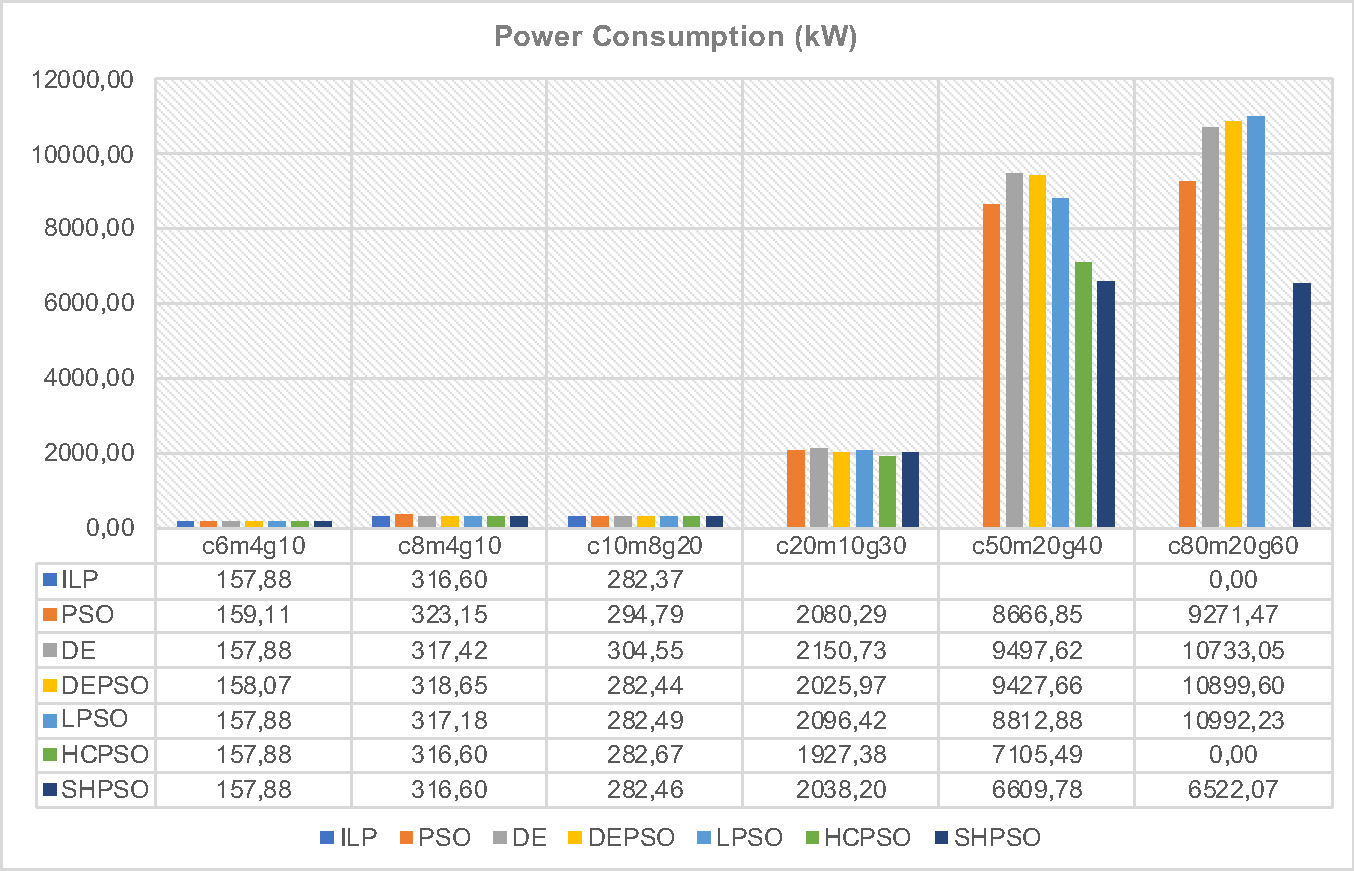
\includegraphics[width=1\linewidth]{img/power_consumption.pdf}
\caption{(Near) Optimal Power Consumption of the Different Software Allocation Problems.}
\label{fig_powerconsumption_ilp_metaheuristic}\vspace{-0.4cm}
\end{figure}

\paragraph{Computation Time} In this context, the computation time is the elapsed time between the start of the optimization and the time at which the fitness value becomes steady, and evaluated for 5000 iterations (or generations). In a way, the computation time also indicates the convergence speed of the best solution. Figure \ref{fig_allocationtime_ilp_metaheuristic} summarizes the computation time of the algorithms for the optimization problems listed in Table~\ref{tbl_samples}. The computation time of \ilp is extremely higher than the rest, which is in the scale of milliseconds for the \pb{6}{10}{4} sample, and in seconds for the \pb{8}{20}{6} and \pb{10}{20}{8}. In the case of the non-hybrid meta-heuristic algorithms, the computation time is in the scale of milliseconds in all of the optimization problems. The computation time of the hybrid \pso{} with the hill-climbing algorithm \hcpso{} got exponential in \pb{50}{20}{40} and returns no solution in the next largest problem. However, the stochastic version of the hill-climbing algorithm returned near optimal solution in $~2sec$ while performing better than the hybrid \pso{} with the differential algorithm \depso, which returned in $\leq 6sec$.
\begin{figure}
\centering
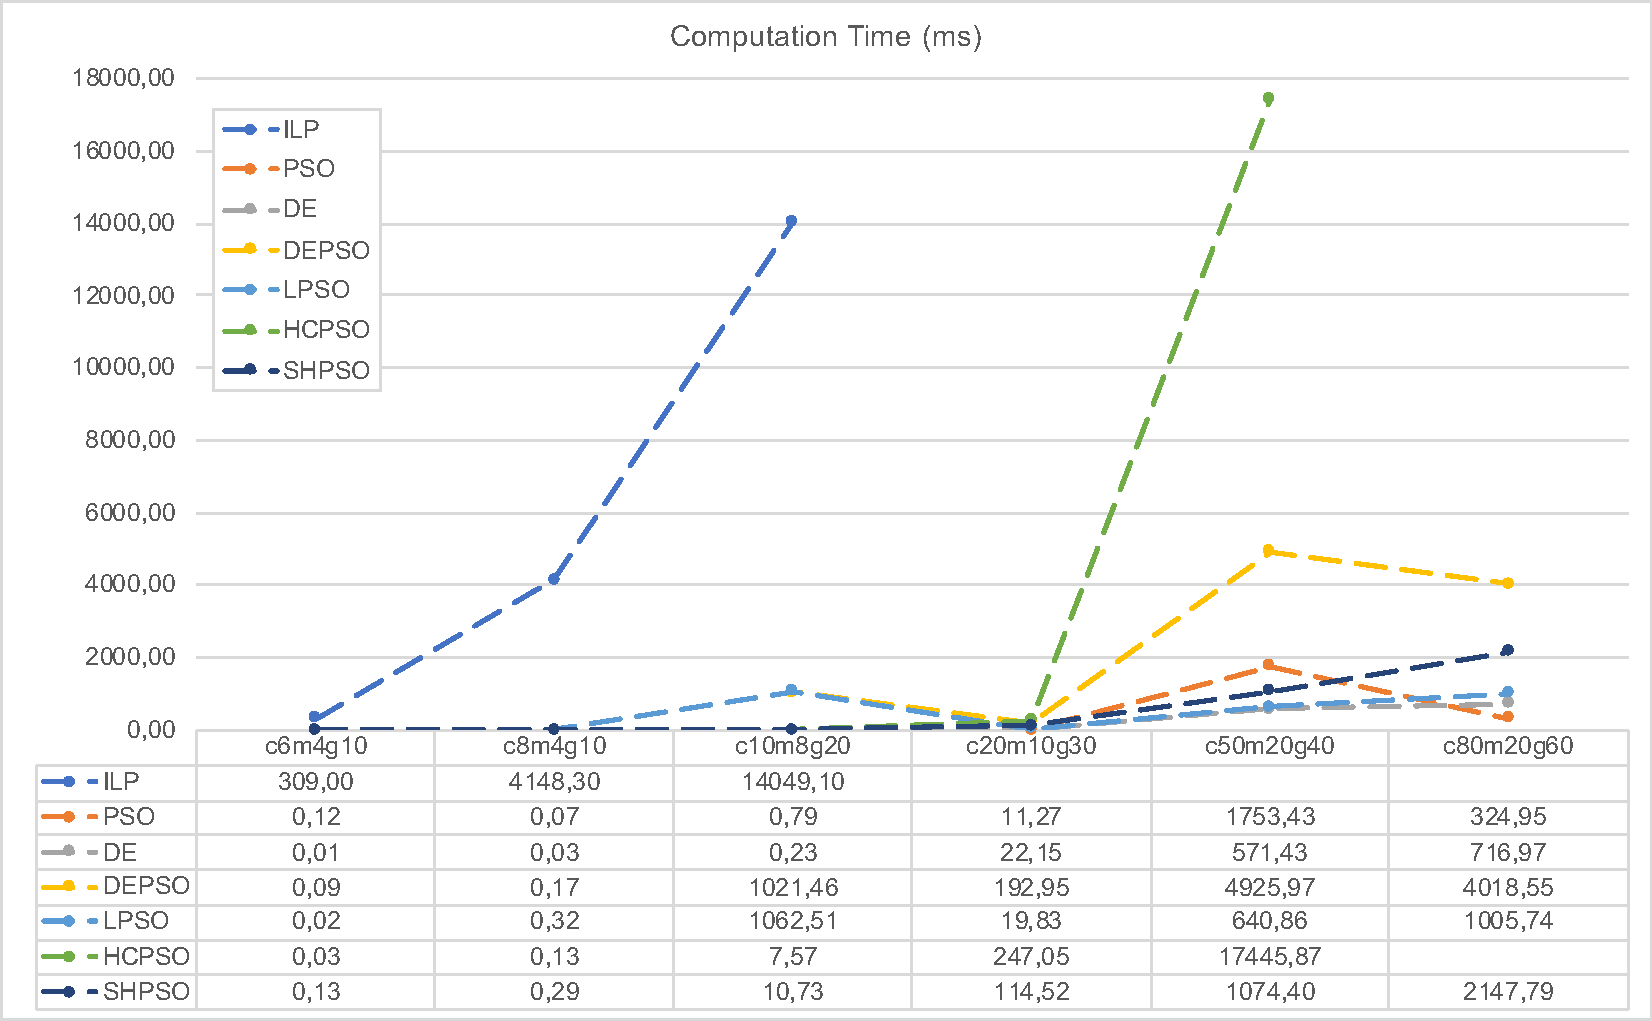
\includegraphics[width=1\linewidth]{img/time_summary.pdf}
\caption{Computation time of the various algorithms for solving different instances of the software allocation problem.}
\label{fig_allocationtime_ilp_metaheuristic}\vspace{-0.4cm}
\end{figure}

\paragraph{Solutions Stability} The \pso{} and \de{} are characterized by random search that facilitates exploration of the search space. However, the randomness also introduces instability of the solutions, that is when the algorithms are executed for the same input, the solutions vary. Such variations are depends on the nature of the algorithms as well as on the optimization problems at hand. In this work, we use  the standard deviation to measure the degree of stability, of the meta-heuristic algorithms. Figure~\ref{tbl_fitness_allocationtime_ilp_plus_metaheuristic} and Figure~\ref{fig_powerconsumption_ilp_metaheuristic} show the deviation of each algorithms from the (near) optimal solutions for the different samples.

Regarding quality of the solutions, the results showed that \hcpso{} is more stable in the first three optimization problems, similarly \de{} and \lpso{} in the first problem. However, as the problem size increases to $g_{10}d_{20}n_8$, the \hcpso{} performed worse while \pso{} and others improve. Regarding computation time, the algorithms become less stable as the problem size increased uniformly for \pso, \de, \hcpso{} and \shpso, however, it is not the case for rest of algorithms.

\subsection{Analysis of Experiment 2}
Figure~\ref{fig_chainsreplicationimprovements} shows results of executing experiment 2, which shows improvements of the computation time by applying the approximation algorithm instead of the exact approach. In the case of the approximation, the delays are exhaustively calculated in the presence of replication. However, the quality of the solutions are degraded as expected due to the approximation. Specifically, the results show $61\%-81\%$ computation time improvement over the exact method while facing quality degradation only for samples $g_{30}d_{3}$ and  $g_{60}d_{2}$. The improvements are in seconds, which implies for a single usage (or run) of the meta-heuristic optimization algorithms, it is not significant. However, considering practical systems design process, which requires several iterations, the commutative effect of the algorithms can negatively impact the responsiveness to engineers. Thus, the improvements can be in trade-off with optimality of the solutions.
\begin{figure}
	\centering
	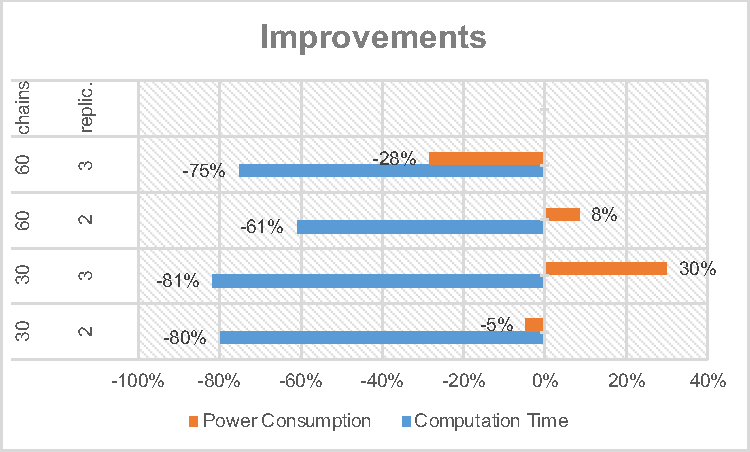
\includegraphics[width=0.7\linewidth]{img/chains_replication_improvements}
	\caption{Effect of approximate algorithm over delay calculations with replication.}
	\label{fig_chainsreplicationimprovements}
\end{figure}

\subsection{Discussion}
The presented software allocation problem considers the complex AUTOSAR system model, which contains AUTOSAR software applications and a network of heterogeneous computing units with respect to power consumption, failure rate and processor speed. The software applications have end-to-end timing and reliability requirements, which are satisfied by effectively and efficiently mapping the software components of the applications to the computing units. We assume the worst-case response time analysis to check the schedulability of the tasks, and age delay analysis to check the schedulability of chains in the system. 

The allocation problem is even more complex since we apply fault tolerance to maximize and subsequently meet the reliability requirements of the applications. The fault tolerance, which is realized by replicating software components, imposes heavy computation on the age delay of the chains. The reliability is computed using state enumeration, which is an exact method, as compared to series-parallel method due to functional inter-dependency between computing units.

Considering the complexity of the system model, the exact method based on the integer-linear programming is limited only to small and medium software allocation problems as shown in Experiment 1. Although, the meta-heuristic algorithms did not always return the optimal solutions, the results are actually very close to the results obtained from \ilp, and the computation time is quite low as compared to the \ilp results.

In terms of optimality, the stochastic hill-climbing performed best next to \ilp which is attributed to the intensive local search of the algorithm. However, it felt short to return near optimal solutions in the largest optimization problem, which is not the case for its stochastic version. Thus, the hybrid \pso{} with the stochastic hill-climbing algorithm relatively more robust, effective and scales well as compared to the rest of the hybridization algorithms.

